% ===== Page 36 =====
\section{Projection Theorem}
\origpage{36}
\begin{theorem}[Hilbert's Projection Theorem]
Let $H$ be a Hilbert space and let $M$ be a finite dimensional subspace of $H$.
For any $x\in H$ the following minimization problem has a solution:
\[
m^* = \arg\min_{m\in M} \norm{x-m}^{2}
\]
\begin{itemize}[nosep]
  \item the exponent $2$ does not matter, the norm is positive;
  \item $\norm{\cdot}$ is the norm induced by the inner product.
\end{itemize}
In other words, we can find the closest vector $m^*$ to $x$ lying in the subspace $M$.
If $m^*$ is a solution, then $x-m^*$ is orthogonal to $M$.
Furthermore, the solution $m^*$ is unique:
\[
m^* = \operatorname{Proj}_M x : \text{ ``Orthogonal Projection of $x$ onto $M$''}
\]
\end{theorem}

\explain{Reminder on $\arg\min$ vs.\ $\min$ (left), and the geometry of the theorem (right).}
\begin{center}
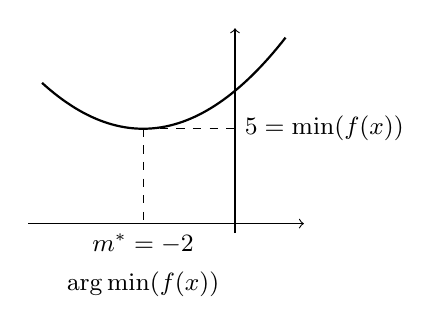
\begin{tikzpicture}
\begin{axis}[
  width=5.2cm, height=4.4cm,
  axis lines=none,
  xmin=-4.6, xmax=1.6, ymin=-1.2, ymax=10.5,
  clip=false]
  \draw[->] (axis cs:-4.5,0) -- (axis cs:1.5,0);
  \draw[->] (axis cs:0,-0.5) -- (axis cs:0,10.3);
  \addplot[thick,domain=-4.2:1.1,samples=60] {0.5*(x+2)^2+5};
  \draw[dashed] (axis cs:-2,5) -- (axis cs:0,5);
  \draw[dashed] (axis cs:-2,5) -- (axis cs:-2,0);
  \node[right,font=\small] at (axis cs:0,5) {$5=\min(f(x))$};
  \node[below,font=\small] at (axis cs:-2,0) {$m^*=-2$};
  \node[font=\small] at (axis cs:-2,-3.2) {$\arg\min(f(x))$};
\end{axis}
\end{tikzpicture}
\qquad\qquad
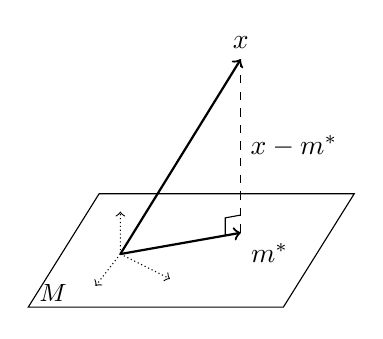
\begin{tikzpicture}[scale=0.9]
  % projection onto plane M
  \draw (0,0) -- (3.6,0) -- (4.6,1.6) -- (1,1.6) -- cycle;
  \node at (0.35,0.2) {\small $M$};
  \coordinate (O) at (1.3,0.75);
  \coordinate (P) at (3.0,1.05);
  \coordinate (X) at (3.0,3.5);
  \draw[->,thick] (O) -- (X) node[above] {$x$};
  \draw[->,thick] (O) -- (P) node[below right] {$m^*$};
  \draw[dashed] (P) -- (X) node[midway,right] {$x-m^*$};
  \draw (3.0,1.3) -- (2.78,1.26) -- (2.78,1.01);
  \draw[->,densely dotted] (O) -- (1.3,1.35);
  \draw[->,densely dotted] (O) -- (0.95,0.3);
  \draw[->,densely dotted] (O) -- (2.0,0.4);
\end{tikzpicture}
\end{center}
\begin{itemize}[nosep]
  \item[$\Rightarrow$] solution exists
  \item[$\Rightarrow$] solution is unique
  \item[$\Rightarrow$] $x-m^*\perp m^*$
\end{itemize}

\sep
\begin{keybox}[width=0.45\linewidth]
$H = M\overset{\perp}{\oplus} M^\perp, \qquad
x = \underbrace{x_1}_{\in M} + \underbrace{x_2}_{\in M^\perp}$
\end{keybox}
\begin{align*}
\norm{x-m}^2 &= \inner{x-m}{x-m} = \inner{x_1+x_2-m}{x_1+x_2-m}\\
&= \big\langle \underbrace{(\underset{\in M}{x_1}-\underset{\in M}{m})}_{\in M} + \underset{\in M^\perp}{x_2},\; (x_1-m)+x_2 \big\rangle\\
&= \inner{x_1-m}{x_1-m} + \underbrace{\inner{\underset{\in M}{x_1-m}}{\underset{\in M^\perp}{x_2}}}_{0} + \underbrace{\inner{x_2}{x_1-m}}_{0} + \inner{x_2}{x_2}\\
&= \norm{x_1-m}^2 + \norm{x_2}^2
\end{align*}
\[
\boxed{m^*=x_1} \text{ to minimize this}
\qquad\Longrightarrow\qquad
\boxed{\therefore\ \min \norm{x-m} = \norm{x_2}}
\]
\begin{itemize}[nosep]
  \item $x_1$ exists
  \item $x_1$ is unique as $M\oplus M^\perp$ is a direct sum property
  \item $x-m^* = x-x_1 = x_2\in M^\perp$
\end{itemize}

\begin{insight}[Why the proof works]
The key identity is the Pythagorean theorem $\norm{x-m}^2 = \norm{x_1-m}^2 + \norm{x_2}^2$, valid because
$x_1-m\in M$ and $x_2\in M^\perp$ are orthogonal. The second term does not depend on $m$, and the first one is
$\ge 0$ with equality \emph{only} for $m=x_1$; this gives existence and uniqueness at once.
The decomposition $H = M\oplus M^\perp$ itself exists because $M$ is finite dimensional: take an orthonormal
basis $\{e_1,\dots,e_k\}$ of $M$ (Gram--Schmidt) and set $x_1=\sum_i \inner{x}{e_i}e_i$, $x_2 = x-x_1$;
then $\inner{x_2}{e_j} = \inner{x}{e_j}-\inner{x}{e_j} = 0$ for every $j$, so $x_2\in M^\perp$.
\end{insight}

\begin{note}
$\V = M^\perp \overset{\perp}{\oplus} M$, \quad $x\in \V$, \quad $x\notin M$.
\[
\R^2 = x\text{ axis} \overset{\perp}{\oplus} y \text{ axis}, \qquad
\R^2 = \underbrace{\Span\left\{\bmat{1\\0}\right\}}_{M} \overset{\perp}{\oplus} \underbrace{\Span\left\{\bmat{0\\1}\right\}}_{M^\perp}
\]
\begin{center}
\begin{tikzpicture}[scale=0.55,baseline=(current bounding box.center)]
  \draw[thick] (-2,0) -- (2.5,0) node[right] {$M$};
  \draw[thick] (0,-2) -- (0,2.5) node[above] {$M^\perp$};
\end{tikzpicture}
\qquad\qquad
$\displaystyle \bmat{1\\2} = \underbrace{\bmat{1\\0}}_{\in M} + \underbrace{\bmat{0\\2}}_{\in M^\perp}$
\end{center}
If a vector is not in $M$, it does not directly mean that it should be inside $M^\perp$. The vector can be written using $M$ and $M^\perp$.
\end{note}

% ===== Page 37 =====
\origpage{37}
\[
x\in M \;\Rightarrow\; m^* = \operatorname{Proj}_M x = x,
\qquad
x = \underbrace{x_1}_{x} + \underbrace{x_2}_{0}: \quad \text{if } x\in M \;\Rightarrow\; \operatorname{Proj}_{M^\perp} x = 0
\]

\begin{example}
$\V=\R^2$, \quad $M=\Span\left\{\bmat{1\\1}\right\}$, \quad $\inner{x}{y} = y\T x$, \quad
$x = \bmat{1\\2}$, \quad $m^* = \operatorname{Proj}_M x$.
\[
m = \alpha\bmat{1\\1} \;\Rightarrow\; m^* = \alpha^*\bmat{1\\1}, \qquad (x-m^*)\perp M
\]
\begin{align*}
x-m^* = \left(\bmat{1\\2} - \alpha^*\bmat{1\\1}\right) &\perp \bmat{1\\1}\\
\bmat{1-\alpha^*\\ 2-\alpha^*} &\perp \bmat{1\\1}\\
1-\alpha^* + 2-\alpha^* = 0 &\;\Rightarrow\; \alpha^* = \tfrac{3}{2}
\end{align*}
\[
\boxed{m^* = \frac{3}{2}\bmat{1\\1}}
\]
\explain{Check: $x-m^* = \bmat{-1/2\\ 1/2}$ and $\bmat{-1/2 & 1/2}\bmat{1\\1} = 0$; the distance from $x$ to $M$ is $\norm{x-m^*} = 1/\sqrt2$.}
\begin{center}
\begin{tikzpicture}[scale=1.1]
  \draw[->] (-1.8,0) -- (2.6,0);
  \draw[->] (0,-1.2) -- (0,2.6);
  \draw[thick] (-1.6,-1.6) -- (2.3,2.3);
  \node[below right] at (-1.6,-1.6) {$M$};
  \node[left] at (0,2) {\scriptsize 2};
  \node[left] at (0,1) {\scriptsize 1};
  \node[below] at (1,0) {\scriptsize 1};
  \draw[->,thick] (0,0) -- (1,2) node[above left] {$x$};
  \draw[dashed] (0,2) -- (1,2);
  \draw[dashed] (1,2) -- (1,0);
  \draw[->,thick,blue!60!black] (0,0) -- (1.5,1.5);
  \node[right] at (1.5,1.4) {$m^*$};
  \draw[dashed] (1,2) -- (1.5,1.5);
  \draw[dashed] (1.5,1.5) -- (1.5,0);
  \draw (1.36,1.36) -- (1.22,1.5) -- (1.36,1.64);
  \node[right] at (1.75,2.65) {$(x-m^*)\perp M$};
\end{tikzpicture}
\end{center}
\end{example}

\begin{example}
\textbf{(1)} $\V$, \quad $M=\Span\{v_1\}$.
\[
m^* = \operatorname{Proj}_M x = \,? \qquad m^* = \alpha^* v_1, \qquad x-m^* = (x-\alpha^* v_1)\perp v_1
\]
\begin{align*}
\inner{x-\alpha^* v_1}{v_1} &= 0\\
\inner{x}{v_1} - \alpha^*\inner{v_1}{v_1} &= 0
\end{align*}
\[
\Rightarrow\quad \alpha^* = \frac{\inner{x}{v_1}}{\inner{v_1}{v_1}}, \qquad m^* = \frac{\inner{x}{v_1}}{\inner{v_1}{v_1}}\cdot v_1
\]

\par\textbf{(2)} $\V$, \quad $M=\Span\{v_1,v_2\}$.
\begin{align*}
m^* &= \operatorname{Proj}_M x = \,?\\
m^* &= \alpha_1^* v_1 + \alpha_2^* v_2\\
(x-\alpha_1^* v_1 - \alpha_2^* v_2)\perp M &\;\Rightarrow\; (x-\alpha_1^* v_1-\alpha_2^* v_2)\perp v_1 \text{ and } v_2
\end{align*}
\begin{align*}
\inner{x-\alpha_1^* v_1-\alpha_2^* v_2}{v_1} = 0 &\;\Rightarrow\; \inner{v_1}{v_1}\alpha_1^* + \inner{v_2}{v_1}\alpha_2^* = \inner{x}{v_1}\\
\inner{x-\alpha_1^* v_1-\alpha_2^* v_2}{v_2} = 0 &\;\Rightarrow\; \inner{v_1}{v_2}\alpha_1^* + \inner{v_2}{v_2}\alpha_2^* = \inner{x}{v_2}
\end{align*}
\[
\underbrace{\bmat{\inner{v_1}{v_1} & \inner{v_2}{v_1}\\[2pt] \inner{v_1}{v_2} & \inner{v_2}{v_2}}}_{\substack{G\\ \text{Gramian Matrix}}}
\underbrace{\bmat{\alpha_1^*\\ \alpha_2^*}}_{\alpha^*}
= \underbrace{\bmat{\inner{x}{v_1}\\ \inner{x}{v_2}}}_{b}
\qquad\Longrightarrow\qquad
G\cdot\alpha^* = b, \quad \boxed{\alpha^* = G^{-1}\cdot b}
\]

% ===== Page 38 =====
\origpage{38}
\begin{align*}
\det G &= \inner{v_1}{v_1}\inner{v_2}{v_2} - \inner{v_1}{v_2}\underbrace{\inner{v_2}{v_1}}_{\overline{\inner{v_1}{v_2}}}\\
&= \inner{v_1}{v_1}\inner{v_2}{v_2} - \abs{\inner{v_1}{v_2}}^2
\end{align*}
\explain{Cauchy--Schwarz: equality satisfied if $v_1=\alpha v_2$; then only in this case $\det G = 0$.}
\[
\det G > 0 \quad \text{if } \underbrace{v_1\neq \alpha v_2}_{\text{linearly indep}}, \qquad
M = \Span\{v_1,v_2\}, \quad m^* = \alpha_1^* v_1 + \alpha_2^* v_2
\]
\begin{insight}
By the Cauchy--Schwarz inequality $\abs{\inner{v_1}{v_2}}^2\le\inner{v_1}{v_1}\inner{v_2}{v_2}$, so always
$\det G\ge 0$, with equality iff $v_1,v_2$ are linearly dependent. Hence for a basis $\{v_1,v_2\}$ of $M$ the
system $G\alpha^*=b$ has exactly one solution, which is the unique $m^*$ promised by the projection theorem.
Note also that $G$ is Hermitian: its $(j,i)$ entry is the complex conjugate of its $(i,j)$ entry.
\end{insight}
\end{example}

\begin{example}
$\V = \{f:[0,1]\to\R\}$, \quad $\displaystyle\inner{f}{g} = \int_0^1 f(t)g(t)\,dt$, \quad
$M=\Span\{1,t\}$, \quad $f(t)=t^2$.

Find $m^* = \operatorname{Proj}_M f$.
\[
v_1(t) = 1, \qquad v_2(t) = t
\]
\begin{align*}
&\underbrace{\bmat{\inner{1}{1} & \inner{t}{1}\\ \inner{1}{t} & \inner{t}{t}}}_{G}\bmat{\alpha_1^*\\ \alpha_2^*} = b = \bmat{\inner{t^2}{1}\\ \inner{t^2}{t}}\\
\Rightarrow\ &\bmat{\int_0^1 dt & \int_0^1 t\,dt\\[4pt] \int_0^1 t\,dt & \int_0^1 t^2\,dt}\bmat{\alpha_1^*\\ \alpha_2^*} = \bmat{\int_0^1 t^2\,dt\\[4pt] \int_0^1 t^3\,dt}\\
\Rightarrow\ &\underbrace{\bmat{1 & 1/2\\ 1/2 & 1/3}}_{G}\bmat{\alpha_1^*\\ \alpha_2^*} = \bmat{1/3\\ 1/4},
\qquad \det G = \frac13 - \frac14 = \frac1{12}\\
&\bmat{\alpha_1^*\\ \alpha_2^*} = \frac{1}{\frac{1}{12}}\bmat{1/3 & -1/2\\ -1/2 & 1}\bmat{1/3\\ 1/4} = \bmat{-1/6\\ 1}
\end{align*}
\[
\boxed{m^* = \operatorname{Proj}_M f = -\frac16 + t}
\]
\[
\norm{f(t)} = \sqrt{\int_0^1 \abs{f(t)}^2\,dt}, \qquad
\min_{m\in M} \norm{\underbrace{t^2}_{x} - m(t)} =
\min_{m(t)\in M} \sqrt{\int_0^1 \abs{t^2-m(t)}^2\,dt}
\]
% note: the "=" between the two minimizations is added for readability (in the notes they are written side by side)
\begin{center}
\begin{tikzpicture}
\begin{axis}[
  width=6.5cm, height=5.5cm,
  axis lines=middle,
  xmin=-0.15, xmax=1.35, ymin=-0.3, ymax=1.4,
  xtick={1}, ytick={1},
  tick label style={font=\scriptsize},
  clip=false]
  \fill[gray!30] (axis cs:0,0) -- plot[domain=0:1,samples=40] (axis cs:\x,{\x*\x}) -- plot[domain=1:0,samples=2] (axis cs:\x,{\x-1/6}) -- cycle;
  \addplot[thick,domain=0:1.1,samples=60] {x^2};
  \addplot[thick,red!60!black,domain=0:1.2,samples=2] {x-1/6};
  \addplot[thick,blue!60!black,domain=0:1,samples=2] {x};
  \draw[densely dotted] (axis cs:0,1) -- (axis cs:1,1);
  \draw[dashed] (axis cs:1,1) -- (axis cs:1,0);
  \node[above left,blue!60!black] at (axis cs:0.45,0.45) {$t$};
  \node[right,red!60!black] at (axis cs:1.2,1.2-1/6) {$m^*=t-\tfrac16$};
  \node[above] at (axis cs:1.1,1.21) {$x=t^2$};
  \node[below left,font=\scriptsize] at (axis cs:0,0) {$0$};
\end{axis}
\end{tikzpicture}
\end{center}
\explain{Shaded: the gap between $t^2$ and its best approximation $m^*$ in $\Span\{1,t\}$.}
\begin{insight}[Checking the answer]
The error $e(t) = t^2-t+\tfrac16$ must be orthogonal to $1$ and $t$:
\begin{align*}
\inner{e}{1} &= \int_0^1 \big(t^2-t+\tfrac16\big)\,dt = \tfrac13-\tfrac12+\tfrac16 = 0,\\
\inner{e}{t} &= \int_0^1 \big(t^3-t^2+\tfrac16 t\big)\,dt = \tfrac14-\tfrac13+\tfrac1{12} = 0. \quad\checkmark
\end{align*}
Since $e\perp m^*$, the minimum error is
$\norm{e}^2 = \inner{e}{t^2} = \tfrac15-\tfrac14+\tfrac1{18} = \tfrac1{180}$, i.e.\
$\min_{m\in M}\norm{t^2-m} = \tfrac{1}{6\sqrt5}\approx 0.075$. So $t-\tfrac16$ is the best straight-line
(least-squares) fit to $t^2$ on $[0,1]$; it crosses $t^2$ at $t=\tfrac12\pm\tfrac{1}{2\sqrt3}$.
\end{insight}
\end{example}

% ===== Page 39 =====
\origpage{39}
\subsection*{General space}
$\V$, $n$ dimensional, \quad $M = \Span\{\underbrace{v_1,v_2,\dots,v_k}_{\text{linearly indep.}}\}$, \quad $k<n$
\[
m^* = \sum_{i=1}^k \alpha_i^* v_i,
\qquad
x-m^* = x-\sum_{i=1}^k \alpha_i^* v_i \;\perp\; v_1, v_2, \dots, v_k
\]
\begin{align*}
\Big\langle x-\sum_{i=1}^k \alpha_i^* v_i,\, v_j\Big\rangle &= 0, \qquad j=1,2,\dots,k\\
\inner{x}{v_j} - \sum_{i=1}^k \alpha_i^*\inner{v_i}{v_j} &= 0
\end{align*}
\[
\underbrace{\bmat{\inner{v_1}{v_1} & \cdots & \inner{v_k}{v_1}\\ \vdots & \ddots & \vdots\\ \inner{v_1}{v_k} & \cdots & \inner{v_k}{v_k}}}_{G}
\underbrace{\bmat{\alpha_1^*\\ \vdots\\ \alpha_k^*}}_{\alpha^*}
= \underbrace{\bmat{\inner{x}{v_1}\\ \vdots\\ \inner{x}{v_k}}}_{b}
\]
$G$ is invertible iff $v_1,\dots,v_k$ are linearly indep. \qquad $\alpha^* = G^{-1}b$
\explain{These $k$ equations are the \emph{normal equations}. $G$ is Hermitian and positive definite for independent $v_i$:
$\beta\Hm G\beta = \norm{\textstyle\sum_i\beta_i v_i}^2 > 0$ for $\beta\neq0$ (written for $\F=\C$ with $G_{ji}=\inner{v_i}{v_j}$).}

\subsection*{Specific Case}
$v_i\perp v_j$ when $i\neq j$: \quad $\{v_1,\dots,v_k\}$ are orthogonal.
\[
\bmat{\inner{v_1}{v_1} & & & 0\\ & \inner{v_2}{v_2} & & \\ & & \ddots & \\ 0 & & & \inner{v_k}{v_k}}
\bmat{\alpha_1^*\\ \vdots\\ \alpha_k^*} = \bmat{\inner{x}{v_1}\\ \vdots\\ \inner{x}{v_k}}
\]
\[
G^{-1}b = \bmat{\dfrac{1}{\inner{v_1}{v_1}} & & 0\\ & \ddots & \\ 0 & & \dfrac{1}{\inner{v_k}{v_k}}}
\bmat{\inner{x}{v_1}\\ \vdots\\ \inner{x}{v_k}}
= \bmat{\dfrac{\inner{x}{v_1}}{\inner{v_1}{v_1}}\\ \vdots\\ \dfrac{\inner{x}{v_k}}{\inner{v_k}{v_k}}}
\]
\[
\alpha_i^* = \frac{\inner{x}{v_i}}{\inner{v_i}{v_i}}, \qquad
\boxed{m^* = \sum_{i=1}^k \frac{\inner{x}{v_i}}{\inner{v_i}{v_i}}\cdot v_i}
\]
For an orthonormal set ($v_i\perp v_j$, $i\neq j$, and $\norm{v_i}=1$):
\[
\boxed{m^* = \sum_{i=1}^k \inner{x}{v_i}\, v_i}
\]

\begin{example}
$\V = \R^{2\times 2}$, \quad $M = \{\text{set of symmetric matrices}\}$
\[
x = \bmat{a & b\\ c & d}, \qquad m^* = \operatorname{Proj}_M x, \qquad \inner{A}{B} = \tr(A\T B)
\]
\begin{align*}
\tr\left(\bmat{a_{11} & a_{21}\\ a_{12} & a_{22}}\bmat{b_{11} & b_{12}\\ b_{21} & b_{22}}\right)
&= \tr\left(\bmat{a_{11}b_{11}+a_{21}b_{21} & \times\\ \times & a_{12}b_{12}+a_{22}b_{22}}\right)\\
&= a_{11}b_{11} + a_{21}b_{21} + a_{12}b_{12} + a_{22}b_{22}
\end{align*}
\[
\norm{A} = \sqrt{\tr(A\T A)} = \sqrt{\inner{A}{A}}
\]
% ===== Page 40 =====
\origpage{40}
\[
\min_{S\ \text{sym.}} \Big(\tr\big[(x-S)\T(x-S)\big]\Big)^{1/2}
\]
\[
M = \Span\Big\{\underbrace{\bmat{1&0\\0&0}}_{v_1},\ \underbrace{\bmat{0&1\\1&0}}_{v_2},\ \underbrace{\bmat{0&0\\0&1}}_{v_3}\Big\}
\]
% corrected: notes had the third label as v_2 (meant v_3)
\explain{$v_1,v_2,v_3$ are mutually orthogonal (no common nonzero entries), so the orthogonal-basis formula $\alpha_i^* = \inner{x}{v_i}/\inner{v_i}{v_i}$ applies.}
\begin{alignat*}{2}
\inner{x}{v_1} &= a, &\qquad \inner{v_1}{v_1} &= 1\\
\inner{x}{v_2} &= b+c, &\qquad \inner{v_2}{v_2} &= 2\\
\inner{x}{v_3} &= d, &\qquad \inner{v_3}{v_3} &= 1
\end{alignat*}
\begin{align*}
m^* &= a\bmat{1&0\\0&0} + \frac{b+c}{2}\bmat{0&1\\1&0} + d\bmat{0&0\\0&1}
= \bmat{a & \frac{b+c}{2}\\ \frac{b+c}{2} & d} = \frac{x+x\T}{2}\\
\operatorname{Proj}_{M^\perp} x &= x-m^* = x - \left(\frac{x+x\T}{2}\right) = \frac{x-x\T}{2}
\end{align*}
\[
\left.\begin{aligned} M &\to 3\text{ dim.}\\ M^\perp &\to 1\text{ dim}\end{aligned}\right\} \;\V \Rightarrow 4\text{ dim}
\]
\begin{insight}
$M^\perp$ is the set of \emph{skew-symmetric} matrices, $M^\perp = \Span\left\{\bmat{0&1\\-1&0}\right\}$:
for $S=S\T$ and $K=-K\T$, $\inner{K}{S} = \tr(S\T K) = \tr(SK) = \tr\big((SK)\T\big) = \tr(K\T S) = -\tr(KS) = -\tr(SK)$,
so $\inner{K}{S}=0$. Thus every square matrix splits uniquely as
$x = \underbrace{\tfrac{x+x\T}{2}}_{\text{symmetric}} + \underbrace{\tfrac{x-x\T}{2}}_{\text{skew-symmetric}}$,
and $\tfrac{x+x\T}{2}$ is the symmetric matrix closest to $x$ in the Frobenius norm $\sqrt{\tr(A\T A)}$.
\end{insight}
\end{example}

\newpage
\subsection{Application of Projection Theorem onto $\C^n$}
$\V=\C^n$, \quad $M = \Span\{m_1,\dots,m_k\}$, \quad $m_i = [\ \ ] \in\C^n$ (column vectors), \quad $x\in\C^n$.
\begin{align*}
m^* &= \operatorname{Proj}_M x = \,?\\
m^* &= P_M\cdot x \quad\Rightarrow\quad P_M\text{: projection matrix onto } M.
\end{align*}
\[
m^* = \alpha_1^* m_1 + \alpha_2^* m_2 + \dots + \alpha_k^* m_k
= \underbrace{\big[\, m_1 \,\vdots\, m_2 \,\vdots\, \cdots \,\vdots\, m_k\,\big]}_{B}
\underbrace{\bmat{\alpha_1^*\\ \alpha_2^*\\ \vdots\\ \alpha_k^*}}_{\alpha^*}
\]
\[
m^* = B\alpha^*, \qquad x-B\alpha^* \perp m_1, m_2, \dots, m_k, \qquad \inner{x}{y} = y\Hm x
\]
% note: "<x,y> = y^H x" is written twice in the notes
\begin{align*}
\inner{x-B\alpha^*}{m_j} = 0 \quad\Leftrightarrow\quad & m_j\Hm(x-B\alpha^*) = 0 \quad\forall j\\
& m_1\Hm(x-B\alpha^*) = 0\\
& \quad\vdots\\
& m_k\Hm(x-B\alpha^*) = 0
\end{align*}
\[
\underbrace{\bmat{m_1\Hm\\ \hline \rule{0pt}{2.8ex}m_2\Hm\\ \hline \rule{0pt}{2.8ex}\vdots\\ \hline \rule{0pt}{2.8ex}m_k\Hm}}_{B\Hm}(x-B\alpha^*) = 0
\qquad\Longrightarrow\qquad
\begin{aligned}
B\Hm(x-B\alpha^*) &= 0\\
B\Hm x - B\Hm B\alpha^* &= 0\\
\underbrace{B\Hm B}_{G}\,\alpha^* &= \underbrace{B\Hm x}_{b}
\end{aligned}
\]

% ===== Page 41 =====
\origpage{41}
\[
\underbrace{\bmat{m_1\Hm\\ \vdots\\ m_k\Hm}}_{B\Hm}
\underbrace{\big[\, m_1 \,\vdots\, m_2 \,\vdots\, \cdots \,\vdots\, m_k\,\big]}_{B}
= \bmat{m_1\Hm m_1 & \cdots & m_1\Hm m_k\\ \vdots & \ddots & \vdots\\ m_k\Hm m_1 & \cdots & m_k\Hm m_k}
= \underbrace{\bmat{\inner{m_1}{m_1} & \cdots & \inner{m_k}{m_1}\\ \vdots & \ddots & \vdots\\ \inner{m_1}{m_k} & \cdots & \inner{m_k}{m_k}}}_{G}
\]
\[
B\Hm x = \bmat{m_1\Hm x\\ m_2\Hm x\\ \vdots\\ m_k\Hm x} = \bmat{\inner{x}{m_1}\\ \inner{x}{m_2}\\ \vdots\\ \inner{x}{m_k}} = b
\]
% corrected: notes had "B x^H = [m_i^H x] = [<x,m_i>] = [Gram matrix]". B x^H is B^H x, and the Gram matrix
% belongs to B^H B (entry (i,j) = m_i^H m_j = <m_j,m_i>), so it was moved to the line above.
\explain{So $B\Hm B\,\alpha^* = B\Hm x$ is exactly the Gram system $G\alpha^* = b$ of the general case, with $\inner{x}{y}=y\Hm x$.}
\begin{align*}
\alpha^* &= (B\Hm B)^{-1}B\Hm x\\
m^* &= B\alpha^*\\
m^* &= \operatorname{Proj}_M x = B(B\Hm B)^{-1}B\Hm x
\end{align*}
\[
\boxed{P_M = B(B\Hm B)^{-1}B\Hm}, \qquad m^* = P_M x
\]
\begin{align*}
P_{M^\perp} &= I-P_M\\
\operatorname{Proj}_{M^\perp} x &= x-\operatorname{Proj}_M x\\
&= x - P_M x = (I-P_M)x
\end{align*}

\sep
% corrected: notes had "P_{M^perp} = (I-P_M) x" (the matrix is I-P_M; (I-P_M)x is the projected vector)
\begin{align*}
P_M\Hm &= \big(B(B\Hm B)^{-1}B\Hm\big)\Hm = B\big((B\Hm B)^{-1}\big)\Hm B\Hm = B(B\Hm B)^{-1}B\Hm = P_M\\
&\Rightarrow\ P_M\Hm = P_M\\
P_M^2 &= P_M\cdot P_M\\
P_M^2 &= B(B\Hm B)^{-1}\cancel{B\Hm B}\,\cancel{(B\Hm B)^{-1}}B\Hm = B(B\Hm B)^{-1}B\Hm = P_M
\end{align*}
\explain{$(B\Hm B)^{-1}$ is Hermitian because $B\Hm B$ is: $\big((B\Hm B)^{-1}\big)\Hm = \big((B\Hm B)\Hm\big)^{-1} = (B\Hm B)^{-1}$.}
% corrected: notes had "B(B^H B^{-1})B^H" in the last step; it is B(B^H B)^{-1}B^H
\[
\boxed{P_M^2 = P_M}
\]
\begin{center}
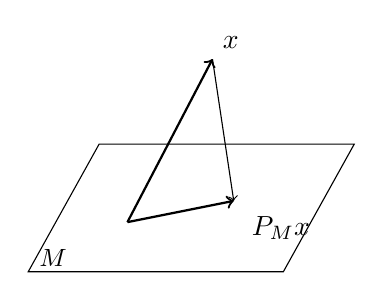
\begin{tikzpicture}[scale=0.9,baseline=(current bounding box.center)]
  \draw (0,0) -- (3.6,0) -- (4.6,1.8) -- (1,1.8) -- cycle;
  \node at (0.35,0.2) {\small $M$};
  \coordinate (O) at (1.4,0.7);
  \coordinate (P) at (2.9,1.0);
  \coordinate (X) at (2.6,3.0);
  \draw[->,thick] (O) -- (X) node[above right] {$x$};
  \draw[->,thick] (O) -- (P);
  \node[below right,xshift=3pt,yshift=-2pt] at (P) {$P_M x$};
  \draw[->] (X) -- (P);
\end{tikzpicture}
\qquad\qquad
$\begin{aligned}
&P_M\cdot P_M x = P_M x\\
&\underline{P_M^2 x = P_M x}
\end{aligned}$
\end{center}

\begin{remark}
An orthogonal projection matrix $P\in\C^{n\times n}$ satisfies
\begin{enumerate}[label=\roman*-), nosep]
  \item $P\Hm = P$
  \item $P^2 = P$ \quad ($P^n = P$)
\end{enumerate}
Also,
\begin{align*}
(I-P)^2 &= I-P\\
(I-P)(I-P) &= I-\cancel{P}-P+\overbrace{P^2}^{\cancel{P}}\\
&= I-P
\end{align*}
\end{remark}
\begin{insight}[Remarks on $P_M$]
\begin{itemize}[nosep]
  \item Conversely, any $P$ with $P\Hm=P$ and $P^2=P$ is the orthogonal projection onto $\Range(P)$:
        $x = Px + (I-P)x$ with $Px\in\Range(P)$, and $(I-P)x\perp\Range(P)$ because
        $(Py)\Hm(I-P)x = y\Hm(P-P^2)x = 0$ for all $y$.
  \item $P_M$ depends only on $M$, not on the chosen basis: if $B' = BT$ with $T$ invertible, then
        $B'(B'^H B')^{-1}B'^H = BT\,T^{-1}(B\Hm B)^{-1}T^{-H}\,T\Hm B\Hm = P_M$.
  \item If the columns of $B$ are orthonormal, $B\Hm B = I$ and $P_M = BB\Hm = \sum_i m_i m_i\Hm$,
        which is the matrix form of $m^* = \sum_i\inner{x}{m_i}m_i$.
  \item $P_M m = m$ for $m\in M$ and $P_M y = 0$ for $y\in M^\perp$ (since $B\Hm y = 0$);
        hence $\Range(P_M) = M$, $\Null(P_M) = M^\perp$.
\end{itemize}
\end{insight}

% ===== Page 42 =====
\origpage{42}
\begin{example}
$\V=\R^3$, \quad $M = \Span\left\{\bmat{1\\1\\1},\bmat{1\\-1\\1}\right\}$, \quad
$x = \bmat{1\\0\\0}$. \quad Find $\operatorname{Proj}_M x = \,?$
\begin{gather*}
B = \bmat{1&1\\1&-1\\1&1}, \qquad
B\T B = \bmat{1&1&1\\1&-1&1}\bmat{1&1\\1&-1\\1&1},\\
B\Hm B = \bmat{3&1\\1&3}, \qquad
(B\Hm B)^{-1} = \bmat{3&-1\\-1&3}\cdot\frac18
\end{gather*}
\begin{align*}
\operatorname{Proj}_M x &= B(B\Hm B)^{-1}B\Hm x = P_M x\\
&= \frac18\bmat{1&1\\1&-1\\1&1}\bmat{3&-1\\-1&3}\underbrace{\bmat{1&1&1\\1&-1&1}\bmat{1\\0\\0}}_{\bmat{1\\1}}\\
&= \frac18\bmat{1&1\\1&-1\\1&1}\underbrace{\bmat{3&-1\\-1&3}\bmat{1\\1}}_{\bmat{2\\2}}\\
&= \frac18\cdot\bmat{4\\0\\4} = \bmat{1/2\\0\\1/2}
\end{align*}
% note: in the notes the three products are shown as nested underbraces under one line
\[
\bmat{1\\0\\0} - \bmat{1/2\\0\\1/2} = \bmat{1/2\\0\\-1/2}
\]
\explain{should be orthogonal to basis vectors (sağlaması için kullanılabilir --- can be used to check the result).}
% Turkish: "can be used to verify (the result)"
\explain{Check: $\bmat{1&1&1}\bmat{1/2\\0\\-1/2} = 0$ and $\bmat{1&-1&1}\bmat{1/2\\0\\-1/2} = 0$ \ $\checkmark$. \
The full matrix is $P_M = \frac18 B\bmat{3&-1\\-1&3}B\T = \frac12\bmat{1&0&1\\0&2&0\\1&0&1}$, whose first column is indeed $\bmat{1/2\\0\\1/2}$.}
\end{example}

\subsection{Application of Projection Theorem into Solutions of Linear Equations}
\[
Ax = b, \qquad A\in\C^{m\times n}, \quad x\in\C^n, \quad b\in\C^m
\]
\begin{center}
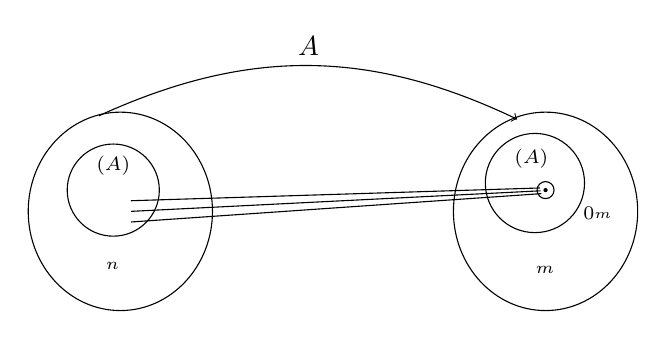
\begin{tikzpicture}[scale=0.9]
  % domain C^n
  \draw (0,0) ellipse (1.3 and 1.4);
  \draw (-0.1,0.3) circle (0.65);
  \node at (-0.1,0.65) {\scriptsize $\Null(A)$};
  \node at (-0.1,-0.85) {\small $\C^n$};
  % codomain C^m
  \draw (6,0) ellipse (1.3 and 1.4);
  \draw (5.85,0.4) circle (0.7);
  \node at (5.8,0.75) {\scriptsize $\Range(A)$};
  \draw (6.0,0.3) circle (0.12);
  \fill (6.0,0.3) circle (0.03);
  \node at (6.75,-0.05) {\scriptsize $0_{\C^m}$};
  % corrected: second small "C^m" label next to the zero vector; read as the subscript of 0 (0_{C^m}), consistent with N(A)={x: Ax=0_{C^m}}
  \node at (6,-0.9) {\small $\C^m$};
  % map
  \draw[->] (-0.3,1.35) to[bend left=25] node[above] {$A$} (5.6,1.3);
  \draw (0.15,0.15) -- (5.92,0.33);
  \draw (0.15,0.0) -- (5.93,0.29);
  \draw (0.15,-0.15) -- (5.94,0.25);
\end{tikzpicture}
\end{center}
\explain{$A$ maps every vector of $\Null(A)$ to $0\in\C^m$.}
\begin{align*}
\Range(A) &= \{y\in\C^m \mid \text{s.t. } \exists x\in\C^n \text{ satisfying } y=Ax\}\\
\Null(A) &= \{x\in\C^n \mid Ax = 0_{\C^m}\}
\end{align*}
\[
\underbrace{\dim(\Range(A))}_{\text{rank}} + \underbrace{\dim(\Null(A))}_{\text{nullity}} = n = \#\text{ of columns of } A
\]
\begin{align*}
&\V = M\overset{\perp}{\oplus}M^\perp\\
&v = v_1+v_2, \qquad v_1\in M, \quad v_2\in M^\perp, \qquad v_1,v_2 \text{ are unique}\\
&v_1\perp v_2, \qquad \dim M + \dim M^\perp = \dim \V
\end{align*}
\begin{enumerate}[label=\arabic*-), nosep]
  \item Is there an exact solution? \ ($\Range(A)$)
  \item If there is, is it unique? \ ($\Null(A)$)
\end{enumerate}
\explain{Question 1 is answered by $\Range(A)\subseteq\C^m$ (the codomain side), question 2 by $\Null(A)\subseteq\C^n$ (the domain side).}

% ===== Page 43 =====
\origpage{43}
\sep
\paragraph{$\bigstar$} $\displaystyle \underbrace{\bmat{1\\1}}_{A}\underset{\in\R}{x} = \underbrace{\bmat{2\\2}}_{b}$,
\qquad $b\in\Range(A)$\\
$\Rightarrow$ $\exists$ an exact solution. \quad $\Rightarrow$ The solution is unique.

\paragraph{$\bigstar$} $\displaystyle \underbrace{\bmat{1\\1}}_{A}x = \underbrace{\bmat{2\\1}}_{b}$
\quad $\Rightarrow$ No exact solution! \qquad $b\notin\Range(A)$
\[
y = Ax = \big[\,a_1 \,\vdots\, a_2 \,\vdots\, a_3 \,\vdots\, \cdots \,\vdots\, a_n\,\big]\bmat{x_1\\x_2\\ \vdots\\ x_n}
= x_1\vec a_1 + x_2\vec a_2 + \dots + x_n\vec a_n
\]
\begin{align*}
\Range(A) &= \Span\{\vec a_1,\vec a_2,\dots,\vec a_n\} \triangleq \text{column space of } A\\
\Range(A) &= \Span\left\{\bmat{1\\1}\right\}, \qquad \bmat{2\\1}\notin\Range(A)
\end{align*}

\begin{keybox}
$\therefore$ 1-) There exists an exact solution \textbf{iff} $b\in\Range(A)$.
\end{keybox}

\paragraph{$\bigstar$} $\displaystyle \underbrace{\bmat{1&2\\1&2}}_{A}\underset{\in\R^2}{x} = \underbrace{\bmat{2\\2}}_{b}$:
\quad $\Range(A) = \Span\left\{\bmat{1\\1}\right\}$ \& $b\in\Range(A)$ $\Rightarrow$ $\therefore\ \exists$ an exact solution
\[
x_1 = \bmat{2\\0} \quad\text{or}\quad x_2 = \bmat{0\\1} \quad\text{or}\quad x_3 = \bmat{4\\-1} \quad\dots
\]

\sep
\[
\left.\begin{aligned}
A &= \bmat{1\\1}, \qquad \dim\C = 1\\
\Range(A) &= \Span\left\{\bmat{1\\1}\right\}, \qquad \dim\Range(A) = 1
\end{aligned}\right\}
\quad
\begin{aligned}
&\underbrace{\dim(\Range(A))}_{1} + \underbrace{\dim(\Null(A))}_{0} = 1 \leftarrow \#\text{ of columns}\\
&\Null(A) = \{0\}, \qquad \dim(\Null(A)) = 0
\end{aligned}
\]

\begin{align*}
&A = \bmat{1&2\\1&2}, \qquad \Range(A) = \Span\left\{\bmat{1\\1}\right\}, \qquad \dim\Range(A) = 1\\
&\underbrace{\dim\Range(A)}_{1} + \underbrace{\dim\Null(A)}_{1} = 2, \qquad
\Null(A) = \Span\left\{\bmat{2\\-1}\right\}
\end{align*}
\[
x_1-x_2 = \bmat{2\\-1}, \qquad x_1-x_3 = \bmat{-2\\1}, \qquad x_2-x_3 = \bmat{-4\\2} \qquad \text{all inside null space.}
\]

\sep
\begin{align*}
&A\hat x = b \qquad \hat x \text{ is exact}\\
&\underset{\substack{\uparrow\\ \in\Null(A)}}{\hat x + m} \;\Rightarrow\; A(\hat x+m) = A\hat x + \underbrace{\overset{\in\Null(A)}{Am}}_{0} = b+0 = b
\end{align*}
% corrected: notes had "= b+0 = 0" at the end (meant "= b") and "x is exact" (meant \hat x)
\begin{itemize}[nosep]
  \item if $\hat x$ satisfies $A\hat x = b$ exactly $\Rightarrow$ $\hat x + m$ satisfies $A(\hat x+m) = b$ exactly \ ($m\in\Null(A)$);
  \item if $m\neq 0 \Rightarrow \hat x \neq \hat x + m$;
  \item if $\Null(A)$ includes nonzero vectors $\Rightarrow$ infinitely many exact solutions.
\end{itemize}

% ===== Page 44 =====
\origpage{44}
\begin{keybox}
$\therefore$ 2-) If an exact solution $\hat x$ exists, then it is unique
$\iff \Null(A) = \{0\}$ \ or \ $\dim\Null(A) = 0$.
\end{keybox}
\begin{insight}
Conversely, if $A\hat x = b$ and $A\tilde x = b$, then $A(\hat x-\tilde x) = 0$, i.e.\ any two exact solutions
differ by a vector of $\Null(A)$. Hence the full solution set is the affine set
$\{\hat x + m : m\in\Null(A)\}$. By rank--nullity, $\Null(A)=\{0\}$ iff $\rank A = n$ (the columns of $A$ are
linearly independent); this requires $m\ge n$.
\end{insight}

\sep
\paragraph{$\bigstar$} $\displaystyle \bmat{1\\1}x = \bmat{2\\1}$, \qquad $Ax = b$, \qquad $b\notin\Range(A)$

\paragraph{Least squares problem:}
\[
\min_{x\in\C^n} \underbrace{\norm{Ax-b}^{2}}_{\text{error}}
\]
\explain{The exponent $2$ doesn't matter; $\norm{\cdot}$ is the induced norm of the inner product.}
\[
\hat x = \arg\min_{x\in\C^n}\norm{Ax-b}
\]
\explain{$\hat x$: minimum error solution / least square solution.}

\begin{align*}
b\in\C^m: \qquad \C^m &= M\overset{\perp}{\oplus}M^\perp\\
\C^m &= \Range(A)\overset{\perp}{\oplus}\Range(A)^\perp
\end{align*}
\[
b = \underset{\in\Range(A)}{b_1} + \underset{\in\Range^\perp(A)}{b_2}
\;\Rightarrow\; b_1 = \operatorname{Proj}_{\Range(A)} b, \quad b_2 = \operatorname{Proj}_{\Range^\perp(A)} b
\;\Rightarrow\; b_1\perp b_2
\]
\begin{align*}
\norm{Ax-b}^2 &= \inner{Ax-b}{Ax-b}\\
&= \big\langle (\underset{\in\Range(A)}{Ax}-\underset{\in\Range(A)}{b_1}) - \underset{\in\Range^\perp(A)}{b_2},\ (Ax-b_1)-b_2\big\rangle
&& (\Range(A) \text{ is a subspace})\\
&= \inner{Ax-b_1}{Ax-b_1}\\
&\quad \cancel{-\inner{Ax-b_1}{b_2}}\\
&\quad \cancel{-\inner{b_2}{Ax-b_1}} && (\to 0 \text{ because of orthogonality})\\
&\quad +\inner{b_2}{b_2}\\
&= \inner{Ax-b_1}{Ax-b_1} + \inner{b_2}{b_2}\\
&= \overbrace{\norm{A\underset{\substack{\uparrow\\ \text{find an } x}}{x}-\underset{\in\Range(A)}{b_1}}^2}^{\text{zero}} + \norm{b_2}^2 \geq \norm{b_2}^2
\end{align*}
% corrected: notes had the first term without the square, i.e. ||Ax-b_1|| + ||b_2||^2
\explain{The first term can be made zero: $b_1\in\Range(A)$, so some $x$ satisfies $Ax=b_1$ exactly.}
\[
\boxed{\min_{x\in\C^n}\norm{Ax-b} = \norm{b_2} = \norm{\operatorname{Proj}_{\Range^\perp(A)} b}}
\]
\[
A\hat x = b_1, \qquad \hat x = \arg\min_{x\in\C^n}\norm{Ax-b}, \qquad
b_1 = \operatorname{Proj}_{\Range(A)} b
\]
\[
\underbrace{\hat x}_{\substack{\text{min error /}\\ \text{least squares solution}}} = \arg\min_{x\in\C^n}\norm{Ax-b}
\]
\begin{insight}[Normal equations]
$A\hat x = b_1$ is equivalent to $b - A\hat x = b_2 \perp \Range(A)$, i.e.\ $a_j\Hm(b-A\hat x) = 0$ for every
column $a_j$ of $A$:
\[
A\Hm(b-A\hat x) = 0 \quad\Longleftrightarrow\quad \boxed{A\Hm A\,\hat x = A\Hm b}
\]
(the same equations as $B\Hm B\alpha^* = B\Hm x$ before, with $B=A$). These normal equations always have a
solution. If the columns of $A$ are linearly independent, $A\Hm A$ is invertible and
$\hat x = (A\Hm A)^{-1}A\Hm b$ is unique; otherwise there are infinitely many least squares solutions,
differing by elements of $\Null(A\Hm A)=\Null(A)$.
\end{insight}

% ===== Page 45 =====
\origpage{45}
\sep
\begin{align*}
&\bmat{1\\1}x = \bmat{2\\1}, \qquad b\notin\Range(A), \qquad \Range(A) = \Span\left\{\bmat{1\\1}\right\}\\
&P_{\Range(A)} = B(B\Hm B)^{-1}B\Hm, \qquad B = \bmat{1\\1}, \qquad B\Hm B = \bmat{1&1}\bmat{1\\1} = 2\\
&P_{\Range(A)} = \bmat{1\\1}\frac12\bmat{1&1} = \bmat{1/2&1/2\\1/2&1/2}\\
&b_1 = P_{\Range(A)}b = \bmat{1/2&1/2\\1/2&1/2}\bmat{2\\1} = \bmat{3/2\\3/2}
\end{align*}
\[
\underbrace{\bmat{1\\1}}_{A}\hat x = \underbrace{\bmat{3/2\\3/2}}_{b_1},
\qquad \hat x = \frac32
\]
\explain{$\hat x = \tfrac32$ is the average of $b = \bmat{2\\1}$.}
\explain{Same result from the normal equations: $A\Hm A = 2$, $A\Hm b = 3$ $\Rightarrow$ $\hat x = \tfrac32$; the minimum error is $\norm{b-b_1} = \norm{\bmat{1/2\\-1/2}} = \tfrac1{\sqrt2}$.}

\paragraph{$\bigstar$} $\displaystyle \bmat{1\\1}x = \bmat{2\\1}$, \qquad
$\Range(A) = \Span\left\{\bmat{1\\1}\right\}$
\[
b_1 = P_{\Range(A)}b = \bmat{1/2&1/2\\1/2&1/2}\bmat{2\\1} = \bmat{3/2\\3/2}
\]
% corrected: notes had the multiplied vector as [1;1] (it is b=[2;1])
\begin{alignat*}{2}
&A\hat x = b_1, &\qquad& \hat x = 3/2\\
&\Null(A) = \{0\},\ \dim\Null(A) = 0 &\qquad& \Rightarrow\ \hat x \text{ is unique.}
\end{alignat*}

\paragraph{$\bigstar$} $\displaystyle \bmat{1&2\\1&2}x = \bmat{2\\1}$, \qquad
$\Range(A) = \Span\left\{\bmat{1\\1}\right\}$, \qquad $b\notin\Range(A)$
\begin{align*}
&b_1 = P_{\Range(A)}b = \bmat{3/2\\3/2}\\
&\bmat{1&2\\1&2}\hat x = \bmat{3/2\\3/2}
\quad\Rightarrow\quad \hat x = \bmat{3/2\\0}, \quad \hat x = \bmat{0\\3/4}, \quad \hat x = \bmat{1/2\\1/2}\\
&\Null(A) = \Span\left\{\bmat{2\\-1}\right\}
\quad\Rightarrow\quad \hat x \text{ is not unique!}
\end{align*}
\explain{All least squares solutions: $\hat x = \bmat{3/2\\0} + t\bmat{2\\-1}$, $t\in\R$ (e.g.\ $t=-\tfrac34$ gives $\bmat{0\\3/4}$, $t=-\tfrac12$ gives $\bmat{1/2\\1/2}$). Each leaves the same error $\norm{b_2} = \tfrac1{\sqrt2}$.}

\sep
\paragraph{Minimum norm solution.}
\[
b\in\Range(A) \;\Rightarrow\; \min_{Ax=b}\norm{x}, \qquad
\hat x_1 = \arg\min_{Ax=b}\norm{x}, \qquad x = \hat x + \overset{\in\Null(A)}{m}
\]
\[
\min_{m\in\Null(A)}\norm{\hat x + m}, \qquad A\hat x = b
\]
\explain{When there are infinitely many solutions, pick the one with the smallest norm. Every solution has the form $\hat x+m$ for one fixed solution $\hat x$, so we minimize over $m\in\Null(A)$.}
\begin{center}
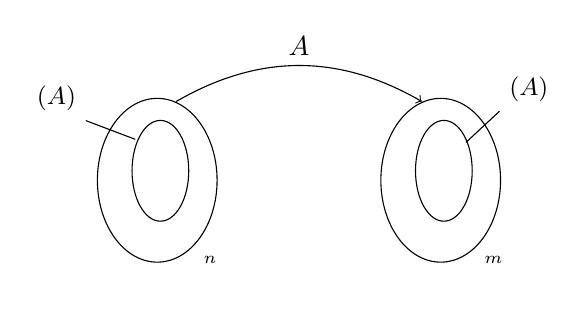
\begin{tikzpicture}[scale=0.8]
  \draw (0,0) ellipse (0.95 and 1.3);
  \draw (0.05,0.15) ellipse (0.45 and 0.8);
  \node at (0.85,-1.35) {\small $\C^n$};
  \node (NA) at (-1.6,1.3) {\small $\Null(A)$};
  \draw (-0.35,0.65) -- (NA.south east);
  \draw (4.5,0) ellipse (0.95 and 1.3);
  \draw (4.55,0.15) ellipse (0.45 and 0.8);
  \node at (5.35,-1.35) {\small $\C^m$};
  \node (RA) at (5.9,1.45) {\small $\Range(A)$};
  \draw (4.9,0.6) -- (RA.south west);
  \draw[->] (0.3,1.25) to[bend left=30] node[above] {$A$} (4.2,1.25);
\end{tikzpicture}
\end{center}
\begin{align*}
&\C^m = \Range(A)\overset{\perp}{\oplus}\Range^\perp(A)\\
&\C^n = \Null^\perp(A)\overset{\perp}{\oplus}\Null(A)\\
&\hat x = \underset{\in\Null^\perp(A)}{\hat x_1} + \underset{\in\Null(A)}{\hat x_2},
\qquad \hat x_1 = \operatorname{Proj}_{\Null^\perp(A)}\hat x, \quad \hat x_2 = \operatorname{Proj}_{\Null(A)}\hat x,
\qquad \hat x_1\perp\hat x_2
\end{align*}

% ===== Page 46 =====
\origpage{46}
\begin{align*}
\norm{\hat x + m}^2 &= \inner{\hat x + m}{\hat x + m}\\
&= \big\langle \underset{\in\Null^\perp}{\hat x_1} + (\underset{\in\Null}{\hat x_2} + \underset{\in\Null}{m}),\ \underset{\in\Null^\perp}{\hat x_1} + (\underset{\in\Null}{\hat x_2} + \underset{\in\Null}{m})\big\rangle\\
&= \inner{\hat x_1}{\hat x_1} + \inner{\hat x_2 + m}{\hat x_2 + m}\\
&= \norm{\hat x_1}^2 + \norm{\hat x_2 + m}^2\\
&\geq \norm{\hat x_1}^2
\end{align*}
\explain{Equality for $m^* = -\hat x_2 \;\Rightarrow\; \norm{\hat x_2 + m} = 0$.}
\[
\min_{\substack{Ax=b\\ m\in\Null(A)}} \norm{\hat x + m} = \norm{\hat x - \hat x_2} = \norm{\hat x_1}
\]
\begin{align*}
A\hat x &= b\\
A(\hat x_1 + \hat x_2) &= b\\
A\hat x_1 + \underbrace{\cancel{A\hat x_2}}_{0} &= b\\
\Rightarrow\quad A\hat x_1 &= b
\end{align*}
\[
\boxed{\hat x_1 = \operatorname{Proj}_{\Null^\perp(A)}\hat x = \text{minimum norm solution}}
\]
\begin{insight}[Summary of the method]
\begin{itemize}[nosep]
  \item $\hat x_1$ does not depend on which solution $\hat x$ we start from: two solutions differ by an element
        of $\Null(A)$, which the projection onto $\Null^\perp(A)$ removes. So the minimum norm solution is unique.
  \item $\Null^\perp(A) = \Range(A\Hm)$ (since $Ax=0 \iff x\perp$ every row of $A$, i.e.\ every column of $A\Hm$).
        Hence the minimum norm solution can be written $\hat x_1 = A\Hm z$, and $AA\Hm z = b$; if $A$ has
        linearly independent rows, $\hat x_1 = A\Hm(AA\Hm)^{-1}b$.
  \item If $b\notin\Range(A)$, combine both steps: replace $b$ by $b_1 = \operatorname{Proj}_{\Range(A)}b$, take any
        least squares solution and project it onto $\Null^\perp(A)$. The result is the \emph{minimum norm least
        squares solution} (this is what the pseudo-inverse $A^{+}b$ computes); the example below does exactly this.
\end{itemize}
\end{insight}

\begin{example}
\[
\bmat{1&2\\1&2}x = \bmat{2\\1}, \qquad
b_1 = \operatorname{Proj}_{\Range(A)} b = \bmat{3/2\\3/2}
\]
\[
\bmat{1&2\\1&2}\hat x = \bmat{3/2\\3/2}
\quad\Rightarrow\quad
\hat x = \bmat{3/2\\0}
\]
\[
\Null(A) = \Span\left\{\bmat{2\\-1}\right\}, \qquad
\underbrace{\dim\Null(A)}_{1} + \underbrace{\dim\Null^\perp(A)}_{=1} = 2
\]
\[
\Null^\perp(A) = \Span\Big\{\underbrace{\bmat{1\\2}}_{v}\Big\} = \Range(A\Hm)
\]
\[
P_{\Null^\perp(A)} = B(B\Hm B)^{-1}B\Hm = \frac{vv\Hm}{v\Hm v}
= \frac{\bmat{1\\2}\bmat{1&2}}{\bmat{1&2}\bmat{1\\2}} = \frac15\bmat{1&2\\2&4}
\]
\[
\hat x_1 = \frac15\bmat{1&2\\2&4}\bmat{3/2\\0} = \frac15\bmat{3/2\\3} = \bmat{3/10\\3/5}
\]
\begin{insight}[Checking the answer]
\begin{itemize}[nosep]
  \item $A\hat x_1 = \bmat{3/10+6/5\\ 3/10+6/5} = \bmat{3/2\\3/2} = b_1$, so $\hat x_1$ is a least squares solution.
  \item $\hat x_1 = \tfrac{3}{10}\bmat{1\\2}\in\Null^\perp(A)$, i.e.\ $\hat x_1\perp\bmat{2\\-1}$.
  \item Starting from $\bmat{0\\3/4}$ or $\bmat{1/2\\1/2}$ instead gives the same $\hat x_1$, e.g.\
        $\tfrac15\bmat{1&2\\2&4}\bmat{0\\3/4} = \bmat{3/10\\3/5}$.
  \item Norms: $\norm{\hat x_1}^2 = \tfrac{9}{20} = 0.45$, smaller than
        $\norm{\bmat{3/2\\0}}^2 = 2.25$, $\norm{\bmat{0\\3/4}}^2 = 0.5625$, $\norm{\bmat{1/2\\1/2}}^2 = 0.5$.
\end{itemize}
\end{insight}
\end{example}
